This chapter identifies the fundamental requirements for converting natural language into structured templates and critically examines existing approaches. The goal is to establish a systematic basis for evaluating current methods and to derive implications for the design of the proposed framework.

\section{Requirements}

This section outlines the core requirements that a system must fulfill to transform natural language input into structured templates with predefined fields. Such templates are widely used across domains, including healthcare (e.g., patient checklists), manufacturing (e.g., quality inspections), and logistics (e.g., delivery reports).

The primary goal of the system presented in this thesis, named Invox, is to support users in filling out these templates more easily, quickly, and accurately. Instead of using traditional tools like a mouse, keyboard, or touchscreen, users interact with the system using natural language. This input can be typed or spoken aloud—both are valid forms of unstructured data. However, it is important to note that voice-based input is just one way of using the system; the true innovation lies in how the system processes and understands natural human language and translates it into structured form data.

In a traditional setting, filling out templates can be tedious. Users must manually locate the correct form, understand what each field is asking for, and type in the responses one by one. This is not only time-consuming but also error-prone. Mistakes may happen due to misunderstandings, skipped fields, or inconsistent use of terminology. The system described in this thesis seeks to overcome these problems by using a multi-agent architecture that processes unstructured input and populates templates automatically using large language models (LLMs).

The motivation behind using LLMs is their strong ability to understand context, infer meaning from loosely structured inputs, and generalize across different domains. When a user gives a voice or text description, the LLMs can interpret what they are trying to say—even if the input is informal, non-linear, or incomplete—and determine how to map this information into the correct fields of a form. This enables users to interact with the system in a more natural and efficient way.

However, building such a system is not straightforward. Several challenges must be addressed to ensure the solution is usable, reliable, and trustworthy across real-world scenarios. To clearly define what such a system should achieve, we identify the following six requirements:   

\textbf{R1 – Consistency:}  
The system must be able to transform heterogeneous and informal input—such as voice transcriptions, chat messages, or handwritten notes—into consistently populated template fields. It should normalize wording, tonality, length, and semantic specificity, and enforce formatting standards so that entries are comparable, unambiguous, and suitable for downstream analysis.  

\textbf{R2 – Information Extraction Abilities:}  
The system should accurately identify and assign relevant details from noisy, fragmented, or multilingual input to the correct fields, while leaving irrelevant fields empty. It must recognize when required information is missing, handle contradictions by prompting for clarification, and integrate scattered fragments into coherent entries.  

\textbf{R3 – Transparency:}  
To foster trust and accountability, the system must make its decision-making process visible. It should highlight the input fragments that support each extracted value and provide confidence scores to indicate the certainty of those values. This enables users to verify outputs efficiently, focus on uncertain cases, and ensure auditability in regulated domains.  

\textbf{R4 – User Correction:}  
The system must enable users to manually edit automatically populated template fields. This ensures immediate error resolution without requiring retraining and empowers users with direct control over the accuracy of the final data submitted.  

\textbf{R5 – Learning and Adaptation:}  
The system should improve over time by consolidating knowledge from past interactions and domain resources. It must learn from manually filled or corrected templates as well as from structured sources such as ontologies, glossaries, or rule sets, progressively reducing repetitive errors and improving alignment with domain-specific practices.

\textbf{R6 – Usability:}  
The system must deliver prompt, near–real-time feedback so interaction feels natural and uninterrupted. This requirement applies to both spoken and typed input (speech is only one use case). Usability is evaluated via end-to-end latency and must be interpreted relative to the declared hardware and deployment profile (e.g., GPU/TPU vs.\ CPU-only, concurrency, network).

These six requirements were identified based on the challenges discussed in Chapter 1 and are supported by current trends in research on natural language processing, speech and text interfaces, and intelligent form-filling systems. Each of the following sections will examine one requirement in detail. We explain what the requirement means, why it matters, and illustrate it with examples. For each requirement, we also define assessment standards that help evaluate how well the system satisfies the requirement in practice.  

\begin{figure}[h!]
    \centering
    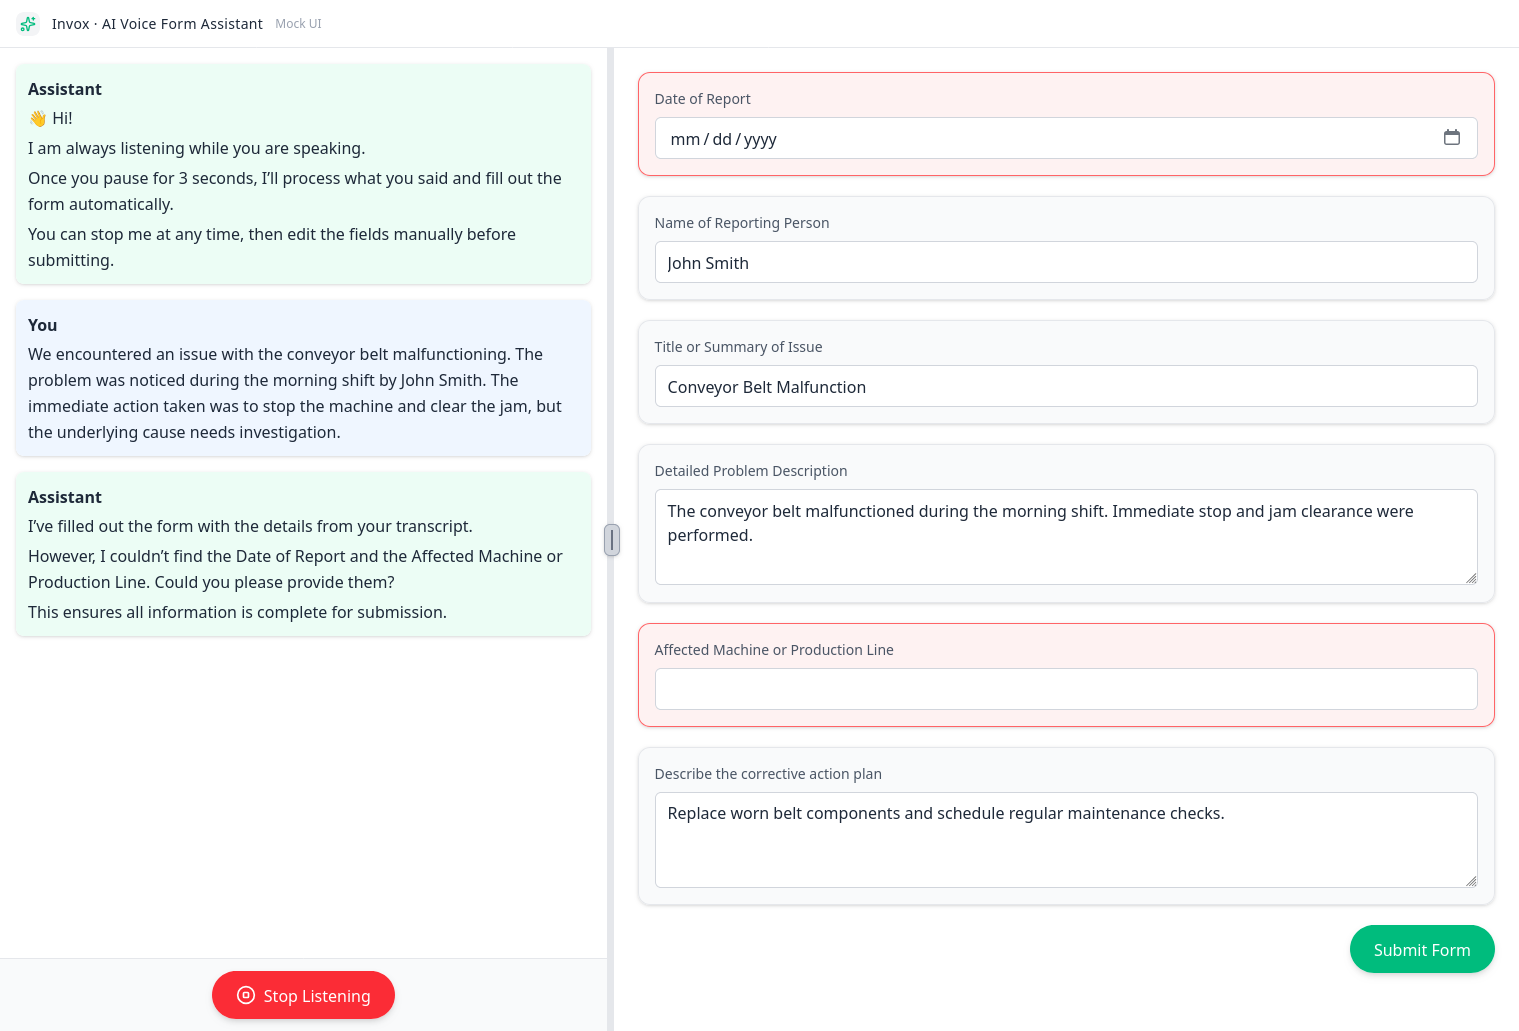
\includegraphics[width=\textwidth]{images/form-filling-example.png}
    \caption{Illustration of the form-filling framework. }
    \label{fig:form-filling-example}
\end{figure}


To make these requirements more concrete, Figure~\ref{fig:form-filling-example} shows a practical usage scenario of the Invox framework. On the left, the user provides a natural language description, which the assistant processes into a structured template on the right. Some fields are automatically filled with extracted values, while others remain highlighted as incomplete and require user clarification. This illustration highlights the central challenges addressed by the requirements: ensuring consistent representation of entries (R1), accurately extracting relevant details (R2), providing transparency about what was filled and why (R3), enabling user correction of missing or incorrect fields (R4), creating a foundation for gradual learning and adaptation over time (R5), and maintaining responsiveness so updates appear promptly during interaction (R6).

\subsection{R1: Consistency}
Consistency refers to the framework’s ability to transform heterogeneous and unstructured inputs—such as transcribed voice recordings, instant messages between employees, or informal written notes—into uniformly populated templates. Unlike free-text logs, templates require values that are standardized and comparable. This means that field entries must not vary arbitrarily in their wording, style, length, or level of specificity. This is a core aspect of what the research field calls "authorship attribution" in the context of LLMs, where the goal is to identify a consistent stylistic "fingerprint" from a given system~\cite{huang2024authorship}. Prior work in conversational systems has shown that a lack of normalization makes it difficult to align user inputs across contexts~\cite{liu2022conversational}, while studies in accessibility highlight how inconsistent representations reduce clarity and comparability for end users~\cite{clark2020accessible}. In the broader NLP field, research on natural language generation similarly stresses that variation without standardization complicates evaluation and downstream analysis~\cite{gatt2018survey}.


As illustrated in Figure~\ref{fig:form-filling-example}, an ideal solution should ensure that once information is extracted, the resulting field values are expressed in a consistent way. This means that answers are not only correct in content but also follow standardized wording, style, formatting, and level of detail. For example, dates should always appear in the same format, technical issues should be described with domain-specific terminology rather than colloquial phrasing, and descriptive fields should provide comparable levels of detail. Such uniform rendering makes entries easier to interpret for humans and more reliable to process automatically across different users, departments, or time periods.


This requirement is especially critical because heterogeneous sources of input inevitably produce inconsistent outputs if left unchecked. In industrial contexts, for example, one technician might describe a machine malfunction as a “slight issue,” another as a “minor fault,” and a third as a “mechanical malfunction.” Even if these phrases describe the same problem, their inconsistency complicates automated reporting and trend analysis, a challenge widely recognized in studies on data quality for industrial systems~\cite{norman2013design}. In healthcare, freeform reports such as “bad cough,” “patient has a cold,” or “respiratory illness” may all refer to the same condition. Medical informatics research has long emphasized that without concept normalization, such variations remain scattered as distinct entries and undermine clinical decision support~\cite{friedman2004survey}. More recent work on clinical text processing shows that mapping expressions to standardized terminologies is essential for interoperability and regulatory compliance~\cite{jonnalagadda2010medical, bodenreider2004unified}. Consistency therefore ensures that all such inputs are aligned to a common representational standard, enabling both human readability and machine-actionable analysis~\cite{shneiderman2016designing}.


In practice, consistency operates across multiple dimensions of representation. At the level of wording, normalization ensures that common phrases are mapped to standardized terminology. For example, “the patient has a cold” can be rendered as “patient with acute nasopharyngitis,” while “the thing is overheating” may be reformulated as “machine component exceeds temperature threshold.” At the level of tonality, consistency harmonizes register and style, replacing subjective or vague expressions such as “slight issue with machine” with standardized formulations such as “minor mechanical malfunction.” At the level of length, overly short entries like “headache” are enriched with sufficient detail to be meaningful, while excessively long descriptions such as “patient reports persistent mild headache for the past two days” are normalized into concise but precise formulations. Finally, at the semantic level, consistency promotes appropriate specificity, ensuring that generic categories like “illness” are consistently replaced with precise terms such as “influenza type B.”  

Formatting and style conventions are equally important to this requirement. Inconsistent formatting creates unnecessary barriers to readability and analysis. For instance, date entries should adhere to predefined standards so that “August 16th” is consistently represented as “08/16/2025.” Similarly, identifiers such as machine codes, patient IDs, or regulatory classification numbers should always follow the same syntactic pattern. Without such formatting alignment, even correctly normalized content may remain ambiguous or unusable across systems. Consistency therefore extends beyond lexical normalization to include structural and formal conventions that guarantee uniformity across the entire template.  

The advantages of consistent template filling are multifold. Consistency improves readability, as users can process and compare entries more quickly when values follow uniform patterns of wording and formatting. It reduces ambiguity by replacing vague or stylistically divergent expressions with precise, standardized equivalents, thereby lowering the risk of misunderstanding. It increases the usefulness of templates in professional contexts, ensuring that field entries are sufficiently detailed to meet regulatory, diagnostic, or legal requirements. Finally, it enhances comparability: homogeneous field values are easier to query, index, and aggregate, which facilitates automated reporting and large-scale data analysis across organizations and timeframes. 

\begin{table}[h!]
\centering
\renewcommand{\arraystretch}{1.6}
\setlength{\tabcolsep}{12pt}
\begin{tabularx}{\textwidth}{|>{\centering\arraybackslash}m{3cm}|>{\arraybackslash}X|}
\hline
\textbf{Visual Score} & \textbf{Interpretation (with thresholds)} \\
\hline
\centering\raisebox{0pt}{\tikz[baseline]{\filldraw[fill=black] (0,0) circle (0.4cm);}} 
& \textbf{High consistency.} Structured fields are correct in most cases (macro exact match/F1 $\geq 0.80$), and free-text fields show strong semantic and stylistic alignment (normalized BLEURT $\geq 0.70$ and Cosine Similarity $\geq 0.70$). \\
\hline
\centering\raisebox{0pt}{\tikz[baseline]{\filldraw[fill=black] (0,0) -- (90:0.4cm) arc (90:-150:0.4cm) -- cycle; \draw (0,0) circle (0.4cm);}} 
& \textbf{Medium consistency.} Structured fields show moderate accuracy (macro exact match/F1 in $[0.65, 0.80)$), and free-text fields achieve moderate semantic and stylistic similarity (normalized BLEURT in $[0.55, 0.70)$ and Cosine Similarity in $[0.55, 0.70)$). \\
\hline
\centering\raisebox{0pt}{\tikz[baseline]{\filldraw[fill=black] (0,0) -- (90:0.4cm) arc (90:-30:0.4cm) -- cycle; \draw (0,0) circle (0.4cm);}} 
& \textbf{Low consistency.} Structured fields are often incorrect (macro exact match/F1 in $[0.50, 0.65)$), and free-text fields align poorly (normalized BLEURT in $[0.40, 0.55)$ and Cosine Similarity in $[0.40, 0.55)$). \\
\hline
\centering\raisebox{0pt}{\tikz[baseline]{\draw (0,0) circle (0.4cm);}} 
& \textbf{No consistency.} Structured accuracy is very low (macro exact match/F1 $<0.50$) and free-text similarity is weak (normalized BLEURT $<0.40$ and Cosine Similarity $<0.40$). Entries are unreliable for comparison or analysis. \\
\hline
\end{tabularx}
\caption{Evaluation scale for R1: Consistency.}
\label{tab:r1-consistency-thresholds}
\end{table}

For evaluation, we use exact match or F1 scores on structured fields such as identifiers, categories, and dates, and BLEURT on free-text fields such as descriptions or notes. Because raw BLEURT scores can vary depending on the checkpoint and dataset, we normalize them to $[0,1]$ across all system outputs in the test set.

To further evaluate the consistency of the system's output style—a key challenge in LLM-generated text—we also employ a stylometric analysis. Specifically, we measure the Cosine Similarity of the n-gram distributions between each system's output and the golden benchmark. Unlike Jaccard similarity, which only considers the presence or absence of n-grams, Cosine Similarity accounts for their frequency. N-grams, which are contiguous sequences of words, provide a quantitative measure of the system's syntactic style. A higher similarity score here indicates that the system's output is not only semantically correct (as measured by BLEURT) but also stylistically aligned with a human-authored standard, thus providing a more comprehensive evaluation of consistency.

To summarize, consistency ensures that heterogeneous, informal, or ambiguous user inputs are transformed into standardized, comparable, and semantically coherent template entries. By enforcing normalization across wording, tonality, length, semantic level, and formatting conventions, and by measuring agreement with the gold standard through exact match for structured fields and BLEURT for free-text fields, the system improves readability, minimizes ambiguity, and ensures that structured data can serve as a reliable foundation for both human decision-making and automated analysis.  
 

\subsection{R2: Information Extraction}
Information extraction refers to the framework’s ability to accurately identify and populate relevant template fields from unstructured or semi-structured input, while leaving irrelevant fields empty. This process goes beyond simple keyword matching and instead relies on linguistic context, entity relationships, and domain-specific semantics to ensure that extracted values are both accurate and meaningful~\cite{grishman1997information, sarawagi2008information}. In practice, information extraction determines whether heterogeneous and noisy inputs—such as partially transcribed voice recordings, multilingual text segments, or fragmented chat messages—can be transformed into reliable structured data~\cite{jurafsky2023speech, liu2022conversational}.  

As illustrated in Figure~\ref{fig:form-filling-example}, an ideal solution must be able to extract relevant details even when input is noisy, fragmented, or multilingual, and populate the corresponding template fields while leaving others empty. The highlighted gaps in the example show that extraction is not only about finding correct values but also about reliably detecting when information is missing and avoiding unsupported guesses.

This requirement matters because real-world text is rarely clean or complete. Voice transcriptions may drop words or introduce errors, employees in international environments may switch between languages mid-sentence, and workplace chat logs often contain fragments, abbreviations, or extraneous commentary~\cite{baldwin2013noisy}. Without strong extraction capabilities, systems risk either leaving critical fields blank or, worse, filling them with incorrect assumptions. In regulated or safety-critical domains such as healthcare or industrial maintenance, such errors can result in compliance violations, misdiagnoses, or operational risks~\cite{radford2023whisper, fathullah2023prompting}.  

Effective extraction must address several challenges simultaneously. First, it must be robust to mixed-language and incomplete input, requiring cross-lingual transfer capabilities for reliable extraction~\cite{ruder2019cross}. A report that states “der Patient… fever since yesterday” combines German and English, yet the system must still detect the symptom and correctly populate the appropriate field. Equally important is recognizing when essential details are missing and preserving empty fields instead of filling them with fabricated values. For example, if a date of inspection is not provided, the system should explicitly leave the field empty rather than guessing. Second, conflict handling is essential. If a transcript contains contradictory information—such as “appointment on August 10” followed by “meeting scheduled for August 12”—the system should not arbitrarily choose one date. Instead, it must detect the inconsistency and prompt the user for clarification, ensuring reliability of the final record. Third, extraction requires contextual understanding. Information is often scattered across multiple parts of a conversation or document, and the system must combine relevant fragments into coherent field values while ignoring unrelated chatter. For instance, if a technician states, “We restarted the press at 23:14. Oh, and the noise got louder after ten minutes,” the system must connect these details to the same inspection event rather than treating them as separate or unrelated entries.  

\begin{table}[h!]
\centering
\renewcommand{\arraystretch}{1.6}
\setlength{\tabcolsep}{12pt}
\begin{tabularx}{\textwidth}{|>{\centering\arraybackslash}m{3cm}|>{\arraybackslash}X|}
\hline
\textbf{Visual Score} & \textbf{Interpretation (based on criteria)} \\
\hline
\centering\raisebox{0pt}{\tikz[baseline]{\filldraw[fill=black] (0,0) circle (0.4cm);}} 
& \textbf{All three criteria satisfied.} The system reliably handles mixed-language and incomplete text, correctly detects and flags conflicts, and successfully integrates related information spread across different text parts. \\
\hline
\centering\raisebox{0pt}{\tikz[baseline]{\filldraw[fill=black] (0,0) -- (90:0.4cm) arc (90:-150:0.4cm) -- cycle; \draw (0,0) circle (0.4cm);}} 
& Two criteria satisfied. For instance, the system handles mixed-language input and detects conflicts but fails to integrate scattered contextual information. \\
\hline
\centering\raisebox{0pt}{\tikz[baseline]{\filldraw[fill=black] (0,0) -- (90:0.4cm) arc (90:-30:0.4cm) -- cycle; \draw (0,0) circle (0.4cm);}} 
& One criterion satisfied. For instance, the system handles mixed-language and incomplete text but fails to detect conflicts and integrate contextual information. \\
\hline
\centering\raisebox{0pt}{\tikz[baseline]{\draw (0,0) circle (0.4cm);}} 
& No criteria satisfied. The system fails to handle mixed-language input, cannot detect conflicts, and does not integrate information spread across different parts of the input. \\
\hline
\end{tabularx}
\caption{Evaluation Scale for R2: Information Extraction Abilities.}
\label{tab:r2-extraction-metrics}
\end{table}


The advantages of strong information extraction capabilities extend across multiple dimensions. They improve accuracy by minimizing both incorrect and missing field values, even when input is fragmented or linguistically complex. They reduce user workload by lowering the amount of manual correction required after automatic field population. They enhance robustness to noise by maintaining performance in the presence of typos, filler words, or irrelevant side remarks. Finally, they enable better multi-source integration by combining relevant information from different segments into a single coherent template entry, which is particularly valuable in collaborative or multi-turn interactions~\cite{shneiderman2016designing}.  

To summarize, information extraction abilities determine whether heterogeneous and noisy user inputs can be reliably transformed into structured templates. A robust system not only identifies and assigns relevant details but also recognizes gaps, resolves contradictions, and integrates scattered fragments into coherent entries. This reduces user workload, improves reliability, and ensures that the extracted data supports both operational decision-making and automated analysis.
 

\subsection{R3: Transparency}
Transparency refers to the framework’s ability to make its decision-making process visible to users by exposing both the evidence behind each extracted value and the system’s level of certainty in that value. Unlike black-box systems that present outputs without explanation, a transparent framework not only shows the populated fields but also reveals the reasoning path by which they were derived. This includes identifying the input fragments that served as evidence and providing explicit indicators of how confident the system is in its interpretations~\cite{doshi2017towards, samek2019explainable}.  

As illustrated in Figure~\ref{fig:form-filling-example}, transparency in an ideal framework means that populated values are never shown in isolation but are accompanied by their supporting evidence and a confidence indicator. The figure highlights how a field such as a date is linked back to the exact phrase in the transcript and annotated with a certainty level, making the reasoning process visible rather than opaque.

This requirement matters because users often interact with template filling systems in high-stakes environments where correctness cannot be taken for granted. In domains such as healthcare, industrial inspection, or compliance reporting, an incorrectly extracted date, measurement, or symptom could lead to operational errors or legal consequences. Without transparency, users are left to either blindly trust the system or manually re-check all outputs. Both outcomes undermine efficiency and adoption. By contrast, when the system highlights the origin of each extracted field and communicates its confidence level, users can selectively verify uncertain or ambiguous entries, thereby improving both trust and productivity~\cite{wang2022trust, ribeiro2016should}.  

In practice, transparency is achieved through two complementary mechanisms. First, source highlighting makes explicit which text fragments in the input led to the population of a given field. For instance, if the transcript contains the phrase “scheduled for 08/16/2025,” the system should highlight this fragment as the evidence for the “Date” field. This allows users to directly trace values back to their textual origins and verify their correctness. Second, confidence scores quantify the system’s certainty about each extracted value. These can be expressed as probabilities (e.g., 0.82 confidence in the extracted date) or as categorical levels (e.g., high, medium, low). Confidence scores help users prioritize where to invest their attention, focusing on entries that are most likely to contain errors while trusting those that are more secure. Together, these mechanisms turn opaque predictions into traceable, verifiable decisions.  

The advantages of transparency are multifold. It builds user trust by establishing a clear link between input data and structured outputs, reducing the perception of the system as a “black box.” It enables efficient error detection, since users can quickly locate uncertain or weakly supported values without re-checking the entire template. Transparency also facilitates training and feedback, as developers and domain experts can identify systematic error patterns by examining low-confidence predictions and their sources~\cite{thomas2019interacting}. Finally, transparency supports compliance in regulated industries by providing auditable evidence trails that show not only what the system decided but also why it decided it.  

\begin{table}[h!]
\centering
\renewcommand{\arraystretch}{1.6}
\setlength{\tabcolsep}{12pt}
\begin{tabularx}{\textwidth}{|>{\centering\arraybackslash}m{3cm}|>{\arraybackslash}X|}
\hline
\textbf{Visual Score} & \textbf{Interpretation} \\
\hline
\centering\raisebox{0pt}{\tikz[baseline]{\filldraw[fill=black] (0,0) circle (0.4cm);}} 
& \textbf{Both criteria satisfied.} The system highlights the exact text fragments that led to each populated field and provides confidence scores for all extracted values. \\
\hline
\centering\raisebox{0pt}{\tikz[baseline]{\filldraw[fill=black] (0,0) -- (90:0.4cm) arc (90:-90:0.4cm) -- cycle; \draw (0,0) circle (0.4cm);}} 
& One criterion satisfied (e.g., confidence scores are displayed but no source highlighting is provided, or vice versa). \\
\hline
\centering\raisebox{0pt}{\tikz[baseline]{\draw (0,0) circle (0.4cm);}} 
& No criteria satisfied. The system provides populated fields without indicating their source or the certainty of extraction, leaving the process opaque. \\
\hline
\end{tabularx}
\caption{Evaluation Scale for R3: Transparency}
\label{tab:r3-transparency}
\end{table}

To summarize, transparency ensures that extracted template values are not only presented as results but also explained in terms of their origins and associated confidence levels. By exposing the reasoning process, the system strengthens user trust, enables efficient verification, and provides the auditability necessary for both iterative improvement and compliance in regulated domains.
 

\subsection{R4: User Correction}
User correction refers to the framework’s ability to allow manual modifications of populated template fields after automatic extraction has taken place. Unlike automated adaptation mechanisms, which rely on system learning from prior interactions, user correction focuses on immediate, explicit interventions that ensure the accuracy of individual outputs. It grants end-users direct control over the final contents of a template, ensuring that errors in recognition, interpretation, or formatting can be addressed before the data is finalized~\cite{bohus2005sorry, shneiderman2016designing}.  

As illustrated in Figure~\ref{fig:form-filling-example}, an ideal framework must let users directly modify any field highlighted as incorrect or uncertain. The figure shows how entries flagged by the system can be overwritten or adjusted before finalization, ensuring that human judgment always has the final word in the template.

This requirement matters because no automated extraction system can achieve perfect accuracy across all input conditions. Transcriptions may introduce errors, ambiguous phrases may be misinterpreted, and domain-specific terminology may be inconsistently mapped. In practical contexts such as medical documentation or maintenance inspections, even small inaccuracies—such as recording the wrong date of an incident or misreporting a measurement—can have disproportionate consequences. By enabling users to directly edit system-generated values, frameworks ensure that such errors can be corrected in real time without the need for retraining, secondary workflows, or downstream data cleaning~\cite{norman2013design}.  

In practice, correction functionality should be applied at the field level. Users must be able to select any automatically populated entry and replace it with the intended value, for example correcting “08/16/2025” to “08/15/2025” in a date field or updating “mechanical failure” to “electrical failure” in an inspection log. Such capabilities not only resolve errors but also give users confidence in the system by demonstrating that the outputs are not immutable black-box predictions. This aligns with broader human–computer interaction principles emphasizing user empowerment, flexibility, and control over system outputs~\cite{shneiderman2016designing, hoy2018voice}.  

The advantages of user correction are twofold. First, it enables immediate error resolution: users do not need to wait for iterative model updates or retraining cycles to address mistakes, but can directly ensure accuracy within the current interaction. Second, it promotes user empowerment by giving individuals ownership of the final data submitted, strengthening their trust in the system and reducing frustration when mistakes inevitably occur. These benefits are particularly important in time-sensitive workflows, where operators must finalize records quickly while retaining the ability to guarantee correctness~\cite{amershi2019guidelines}.


\begin{table}[h!]
\centering
\renewcommand{\arraystretch}{1.6}
\setlength{\tabcolsep}{12pt}
\begin{tabularx}{\textwidth}{|>{\centering\arraybackslash}m{3cm}|>{\arraybackslash}X|}
\hline
\textbf{Visual Score} & \textbf{Interpretation} \\
\hline
\centering\raisebox{0pt}{\tikz[baseline]{\filldraw[fill=black] (0,0) circle (0.4cm);}} 
& \textbf{Full correction support.} Users can edit any populated field directly, ensuring complete control over the final template. \\
\hline
\centering\raisebox{0pt}{\tikz[baseline]{\draw (0,0) circle (0.4cm);}} 
& \textbf{No correction support.} Automatically populated values cannot be modified by users, leaving inaccuracies unresolved. \\
\hline
\end{tabularx}
\caption{Evaluation Scale for R4: User Correction}
\label{tab:r4-correction}
\end{table}

To summarize, user correction ensures that populated templates remain accurate by enabling individuals to directly edit extracted values. This requirement emphasizes immediate error resolution and user empowerment, giving people control over final outputs while reinforcing trust in the system’s reliability.


\subsection{R5: Learning and Adaptation}
Learning and adaptation refer to the framework’s ability to improve its performance over time by incorporating knowledge from user interactions, corrections, and structured domain information. Unlike static systems, which produce the same outputs regardless of experience, an adaptive framework evolves continuously. It refines its internal models and decision-making strategies based on provided examples, explicit corrections, and formal domain rules, thereby becoming more accurate and contextually aligned with the environment in which it is deployed~\cite{doshi2017towards, sun2023slot}.  

As illustrated in Figure~\ref{fig:form-filling-example}, finalized corrections and domain glossaries feed a feedback loop that informs future fills. This matters because using both sources reduces recurring errors and steadily improves accuracy.

This requirement matters because template filling systems are often deployed in highly specialized settings where general-purpose models cannot fully capture local terminology, workflows, or conventions. For example, a healthcare provider may require specific mappings between colloquial expressions such as “chest cold” and formal diagnostic categories, while a manufacturing plant may use internal identifiers or shorthand that differ from industry-wide terminology. Without learning and adaptation, the system risks repeating the same mistakes indefinitely, requiring users to make the same corrections again and again. By contrast, a system that consolidates knowledge from past interactions and domain inputs progressively reduces error rates and builds long-term efficiency~\cite{liu2022conversational, mialon2023augmented}.  

In practice, adaptation can occur through two complementary mechanisms. First, learning from provided filled-in templates allows the system to build expectations about the type and structure of values that belong in each field. For example, if historical forms consistently show that an employee ID consists of exactly five characters, the system can detect when a user provides only three and prompt them to complete the entry correctly. Over time, such feedback reduces recurring formatting or completeness errors by aligning new inputs with established patterns. Second, learning from domain knowledge integrates structured resources such as ontologies, glossaries, or formal rule sets. For instance, a medical ontology may specify that “flu” and “influenza” are synonymous terms, while an engineering glossary may define acceptable formats for torque values. By encoding such knowledge, the system improves both extraction and formatting, aligning outputs with established standards rather than ad-hoc interpretations~\cite{clark2020accessible, chen2024webforms}.

The advantages of learning and adaptation are cumulative. Accuracy improves progressively as the system incorporates examples and corrections, ensuring that the framework becomes more reliable the longer it is used in a given domain. Knowledge consolidation ensures that corrections made once benefit future cases, reducing the burden of repetitive manual adjustments. Continuous refinement also lowers the risk of systematic errors, as patterns of mistakes are gradually eliminated. These capabilities transform template filling from a static tool into an evolving system that adapts to organizational needs and grows more effective with sustained use~\cite{shneiderman2016designing, amershi2019guidelines}.  

\begin{table}[h!]
\centering
\renewcommand{\arraystretch}{1.6}
\setlength{\tabcolsep}{12pt}
\begin{tabularx}{\textwidth}{|>{\centering\arraybackslash}m{3cm}|>{\arraybackslash}X|}
\hline
\textbf{Visual Score} & \textbf{Interpretation} \\
\hline
\centering\raisebox{0pt}{\tikz[baseline]{\filldraw[fill=black] (0,0) circle (0.4cm);}} 
& \textbf{Both mechanisms satisfied.} The system learns from corrected or manually filled templates and incorporates structured domain knowledge such as ontologies and glossaries. \\
\hline
\centering\raisebox{0pt}{\tikz[baseline]{\filldraw[fill=black] (0,0) -- (90:0.4cm) arc (90:-90:0.4cm) -- cycle; \draw (0,0) circle (0.4cm);}} 
& One mechanism satisfied (e.g., the system learns from corrections but cannot integrate domain knowledge, or vice versa). \\
\hline
\centering\raisebox{0pt}{\tikz[baseline]{\draw (0,0) circle (0.4cm);}} 
& No mechanisms satisfied. The system is static, with no ability to learn from past usage or structured knowledge sources. \\
\hline
\end{tabularx}
\caption{Evaluation Scale for R5: Learning and Adaptation}
\label{tab:r5-learning}
\end{table}

To summarize, learning and adaptation ensure that the framework evolves with use, incorporating both user-provided corrections and structured domain knowledge. This capability reduces repetitive errors, consolidates expertise, and progressively improves accuracy, enabling the system to remain aligned with the specialized needs of its deployment context.


\subsection{R6: Usability}
\subsection*{R6: Usability}

Usability in the context of this framework refers primarily to \textbf{latency}, i.e., the time delay between user input and the system’s output (e.g., updated template fields becoming visible). While this thesis evaluates a speech-driven scenario, \emph{speech is only one use case}; the core task is the transformation of \emph{unstructured input (spoken or typed text)} into structured templates. Accordingly, the latency requirement applies to any unstructured-to-template pipeline (typed submissions, transcripts, or mixed modalities). In such settings, responsiveness directly determines whether interaction feels natural and uninterrupted. Human–computer interaction research consistently shows that feedback within two to three seconds is perceived as natural turn-taking, while longer delays disrupt concentration and diminish trust in the system~\cite{shneiderman2016designing}. For voice-first applications, user expectations are shaped by everyday experiences with assistants, where near-instantaneous responses are the norm~\cite{wang2021slu}.

As illustrated in Figure~\ref{fig:form-filling-example}, the template should update promptly after a spoken or typed submission. Timely visual feedback preserves flow and enables quick verification.

Unlike accuracy or error tolerance, which are covered in other requirements (R1–R5), usability here is scoped strictly to latency. This requirement matters because template filling often occurs in time-pressured contexts (e.g., hospitals or industrial facilities), where long waiting times interrupt workflows. For example, a technician dictating a machine fault—or a clerk pasting a long free-text note—must continue seamlessly; if the system takes ten or more seconds to update, the reporting process is disrupted and efficiency drops. Thus, latency is the decisive factor for adoption in real-world deployments.

However, latency is not an absolute property of the software alone. It is strongly influenced by the \textbf{hardware and deployment environment} on which inference is performed. High-performance accelerators such as GPUs and TPUs can significantly reduce end-to-end response time, whereas CPU-only or resource-constrained devices typically increase delays~\cite{shneiderman2016designing, jurafsky2023slp}. Therefore, when evaluating usability, latency benchmarks must always be reported together with the hardware profile (e.g., GPU/TPU type, number of concurrent users, and network setting). This ensures that usability scores are interpreted relative to realistic deployment contexts rather than as abstract performance claims.

\begin{table}[h!]
\centering
\renewcommand{\arraystretch}{1.6}
\setlength{\tabcolsep}{12pt}
\begin{tabularx}{\textwidth}{|>{\centering\arraybackslash}m{3cm}|>{\arraybackslash}X|}
\hline
\textbf{Visual Score} & \textbf{Interpretation} \\
\hline
\centering\raisebox{0pt}{\tikz[baseline]{\filldraw[fill=black] (0,0) circle (0.4cm);}} 
& \textbf{High usability.} p95 end-to-end (E2E) latency $\leq$ 3\,s on the declared hardware profile. Interaction feels natural; conversational pacing is preserved. \\
\hline
\centering\raisebox{0pt}{\tikz[baseline]{\filldraw[fill=black] (0,0) -- (90:0.4cm) arc (90:-90:0.4cm) -- cycle; \draw (0,0) circle (0.4cm);}}
& \textbf{Medium usability.} p95 E2E latency in $(3,10)$\,s. Delay is noticeable but tolerable in most workflows. \\
\hline
\centering\raisebox{0pt}{\tikz[baseline]{\draw (0,0) circle (0.4cm);}} 
& \textbf{No usability.} p95 E2E latency $>$ 10\,s or frequent timeouts. Workflow is impractical under this configuration. \\
\hline
\end{tabularx}
\caption{Evaluation Scale for R6: Usability}
\label{tab:r6-usability}
\end{table}

\paragraph{Evaluation method (latency definition).}
We measure \emph{end-to-end (E2E) latency} from the time the user finishes an utterance \emph{or submits text} until the corresponding template fields are rendered. For each system, p95 latency is reported (optionally p50 for typical-case summaries), ensuring responsiveness is captured consistently~\cite{amershi2019guidelines, jurafsky2023slp}. All results must specify the underlying hardware setup.

To summarize, usability in this framework is defined as responsiveness measured through latency for unstructured-to-template conversion across modalities (speech and text). Because latency is hardware-dependent, evaluation must always contextualize results by reporting the target infrastructure. This ensures comparability across systems while keeping interpretations grounded in practical deployment realities.



\section{Related Work}

The transformation of unstructured natural language into structured templates represents a fundamental challenge in natural language processing that intersects multiple research domains. This challenge has gained renewed attention with the advent of large language models (LLMs), which demonstrate unprecedented capabilities in understanding context, extracting relevant information, and generating structured outputs from free-form text. 

However, despite these advances, current approaches often struggle with the specific requirements identified in Section 2.1, particularly when dealing with noisy, domain-specific, or incomplete inputs common in real-world industrial and professional settings.
This section examines the current state of research relevant to multi-agent template filling systems, with particular focus on how existing approaches address the core challenges of consistency, information extraction accuracy, transparency, user correction capabilities, learning mechanisms, and usability. The analysis reveals significant gaps in current methodologies, particularly in their monolithic design assumptions and limited adaptability to specialized domains.

The review is organized into four key areas that directly inform the design of the proposed Invox system. First, we examine traditional and modern approaches to template filling and structured information extraction, tracing the evolution from rule-based systems to contemporary LLM-driven methods. Second, we analyze prompt engineering techniques that have emerged as critical tools for guiding LLMs toward structured output generation. Third, we explore multi-agent LLM systems that decompose complex tasks into specialized components, offering potential solutions to the modularity and transparency challenges identified in monolithic approaches. Finally, we evaluate how existing solutions perform against the six requirements established in this thesis, identifying specific limitations that motivate the need for a more comprehensive, modular approach to speech-driven template filling.


\subsection{Template Filling and Structured Information Extraction}
Extracting structured information from unstructured text has been a central challenge in natural language processing (NLP) for decades. Early systems were rule-based, using handcrafted grammars, dictionaries, and regular expressions to detect domain-specific patterns \cite{grishman1997information}. These methods worked well in narrow settings but were brittle, required heavy manual effort, and could not easily adapt to new domains.

Statistical models offered more flexibility. Hidden Markov Models (HMMs) were used to model sequential dependencies, while Conditional Random Fields (CRFs) became particularly influential by enabling richer feature-based sequence labeling \cite{sarawagi2008information}. CRFs were widely adopted for tasks such as Named Entity Recognition (NER) and slot filling, achieving strong results on shared tasks like CoNLL-2003 \cite{tjong2003introduction}. Despite these advances, statistical models still struggled with domain transfer, long-range dependencies, and their reliance on handcrafted features.

Another important limitation of early work was the reliance on pipeline-based architectures. Classical information extraction was usually divided into subtasks such as entity recognition, relation classification, and template alignment. Each stage depended on the output of the previous one, which often led to error propagation \cite{jurafsky2023speech}. For example, if the entity recognition module mislabeled an organization, that error would carry over to relation classification and template population. While pipelines offered modularity, they lacked robustness and transparency, making them hard to apply in noisy or domain-specific environments.

A major breakthrough came with the transformer architecture \cite{vaswani2017attention}. Transformers introduced self-attention and large-scale pretraining, which made it possible to capture long-range context and resolve ambiguity in ways earlier models could not. Building on this foundation, large language models (LLMs) can now generate structured outputs directly, for example in JSON, XML, or task-specific templates. This has enabled information extraction to be performed in zero-shot or few-shot settings, significantly reducing the need for task-specific labeled data \cite{brown2020language,wei2022emergent}. This marks a shift from extractive, pipeline-based designs to generative, end-to-end systems.

One influential contribution in this direction is the work of Du, Rush, and Cardie on \textit{Template Filling with Generative Transformers} \cite{du2021template}. Their framework replaces the traditional two-step pipeline of NER followed by event classification with a single generative system. The model conditions on document tokens and event type markers to generate slot fillers directly. This design captures dependencies across multiple events in one document, avoiding the error propagation typical of pipelines. On the MUC-4 dataset, their approach outperformed both pipeline-based and extractive neural baselines, especially for documents that described multiple events.

\begin{figure}
    \centering
    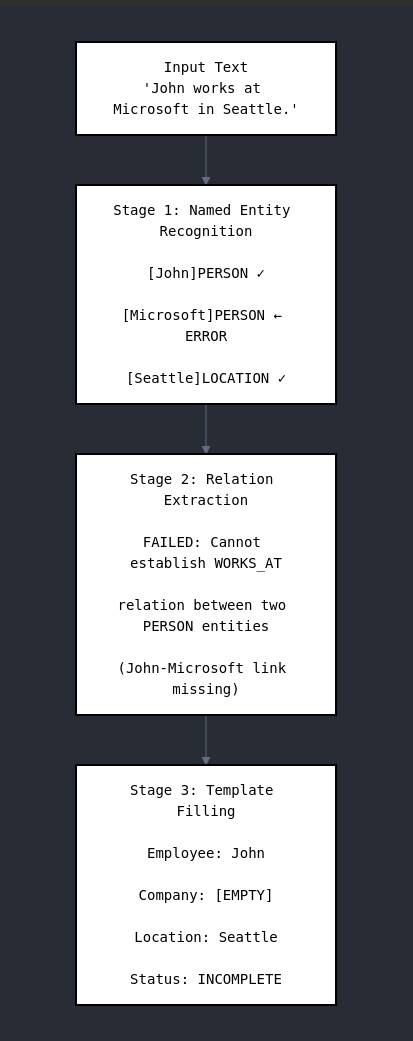
\includegraphics[width=0.6\linewidth]{images/error_propagation.png}
    \caption{Error Propagation Illustration}
    \label{fig:placeholder}
\end{figure}

Benchmarks have played a crucial role in driving research in this area. The MUC-4 dataset \cite{chinchor1992muc} defined an early template filling task for terrorism-related news reports. The ACE program \cite{doddington2004ace} expanded the scope by introducing entity, relation, and event extraction benchmarks across domains. CoNLL-2003 \cite{tjong2003introduction} provided a widely used benchmark for NER in English and German newswire. More recently, speech-based datasets such as SLURP \cite{bastianelli2020slurp} have enabled evaluation of spoken language understanding and slot filling. These benchmarks revealed both the strengths and weaknesses of successive methods, showing where statistical approaches failed and where generative models improved performance. However, they also highlighted the limitations of surface-level metrics such as precision, recall, and F1, which do not capture issues like consistency or robustness.

Despite these advances, domain-specific challenges remain. In healthcare, systems must handle specialized terminology, abbreviations, and implicit knowledge that may not be stated explicitly \cite{friedman2004survey}. In manufacturing and industrial contexts, extraction is complicated by technical identifiers, inconsistent documentation, and informal reporting styles often found in shift logs or maintenance notes \cite{wang2021slu}. These domains require systems that combine robustness with adaptability to diverse forms of domain language.

Work on speech-driven template filling has also emerged. Sun et al.\ study \textit{Speech-based Slot Filling using Large Language Models} \cite{sun2023slot}, focusing on the task of extracting slot values from automatic speech recognition (ASR) transcriptions under noisy conditions. Their evaluation of GPT-3.5, GPT-4, LLaMA, and Vicuna on the SLURP dataset introduces techniques such as structured prompt design, noise-robust LoRA fine-tuning, and linearised knowledge injection (LKI). Their findings show that while LLMs generalize well in zero-shot and few-shot settings, robustness in real-world speech requires careful prompt design and adaptation strategies. This is particularly relevant for this thesis, which addresses speech-based template filling.

Practical tools are also emerging. LangExtract, developed by Google, provides a schema-based information extraction framework using LLMs \cite{google2024langextract}. It maps unstructured text into user-defined JSON schemas, demonstrating how schema-constrained prompting can be deployed in production. However, it relies on a single model, does not support modular correction or consensus across multiple models, and offers limited transparency since intermediate reasoning steps are not exposed.

LLMs have also been applied to structured generation beyond classical information extraction. Chen et al.\ propose \textit{Automated Web Application Testing with LLMs and Screen Transition Graphs} \cite{chen2024webforms}. Their method combines structural graphs of websites with LLM-based generation of Selenium test scripts. Screen transition graphs capture navigation flows, while state graphs represent conditional forms. The LLM then produces executable test cases consistent with these constraints. Although applied in a different domain, this work illustrates the broader applicability of schema-constrained structured generation.

A related line of work focuses on schema enforcement and output alignment. Since LLMs are generative, their outputs can be inconsistent or deviate from the expected template format. Methods such as constrained decoding for structured prediction \cite{anderson2017guided}, schema-guided prompting \cite{zhang2023sgptod}, and external schema validation have been proposed to reduce these issues. These techniques are especially important in regulated or safety-critical domains like healthcare and industry, where outputs must adhere strictly to predefined schemas.

Overall, the field has progressed from rule-based systems, to statistical models, and now to transformer-based generative architectures. Each step has improved the ability to handle complex, ambiguous, and domain-specific data. At the same time, current methods share a key dependency: their success often hinges on careful prompt design and schema specification. This makes prompt engineering a crucial part of ensuring that LLMs consistently generate structured outputs aligned with user requirements. The next subsection therefore examines prompt engineering strategies for information extraction and template filling in greater detail.


\subsection{Prompt Engineering for Information Extraction}
Large language models can generate structured outputs, but their reliability often depends on how the task is presented to them. Prompt engineering has therefore become a central technique. By carefully designing instructions, examples, and schema descriptions in the prompt, users can guide LLMs to align their generative outputs with the structured requirements of template filling.

The idea that LLMs can adapt to new tasks without retraining was first demonstrated through in-context learning. Brown et al.\ showed that GPT-3 could perform unseen tasks when given only a natural language description and a few examples \cite{brown2020language}. Later studies such as Wei et al.\ explored the so-called “emergent abilities” of LLMs, where models suddenly demonstrate strong zero-shot and few-shot performance once they reach a certain scale \cite{wei2022emergent}. For information extraction, this means that a model can often fill structured fields if the prompt specifies the task and provides one or two demonstrations.

Designing effective prompts, however, is not straightforward. Sun et al.\ \cite{sun2023slot} propose structured prompts for speech-based slot filling that include task definitions, slot descriptions, and linearized external knowledge. Their experiments show that such prompt structures make LLMs more robust to noise in automatic speech recognition (ASR) transcripts. Similarly, Lin et al.\ \cite{lin2021leveraging} show that including slot descriptions directly in prompts improves zero-shot dialogue state tracking, since it grounds the model in the meaning of each field. These studies highlight how prompts can embed domain knowledge and ontology definitions to improve extraction quality.

The choice between zero-shot and few-shot prompting also affects performance. Zero-shot prompts rely only on schema descriptions, which makes them flexible but often less reliable. Few-shot prompting, where carefully selected input–output examples are added to the prompt, improves consistency but comes at the cost of longer prompts and higher inference latency. Pan et al.\ \cite{pan2023chatgpt} evaluated ChatGPT for dialogue understanding and found that few-shot prompting consistently outperformed zero-shot in accuracy, though response times increased.

\begin{figure}
    \centering
    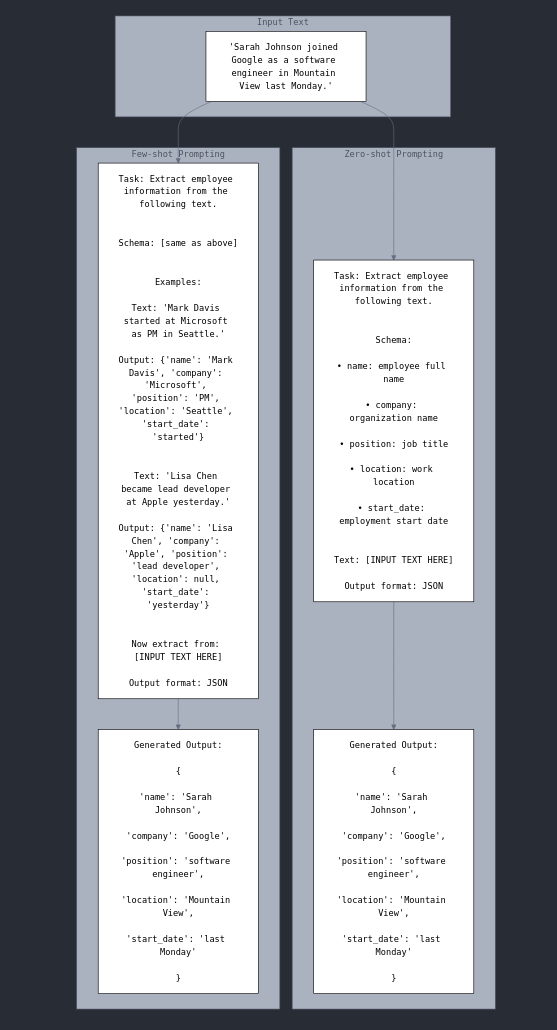
\includegraphics[width=0.8\linewidth]{images/zero_shot_vs_few_shot.png}
    \caption{Zero-shot vs Few-shot Prompting for Template Filling}
    \label{fig:placeholder}
\end{figure}

Schema-constrained prompting has also been investigated as a way to enforce output structure. Zhang et al.\ \cite{zhang2023sgptod} introduced SGP-TOD, where prompts embed schema definitions for task-oriented dialogue systems. By instructing the model to generate only values that fit the schema, they reduced invalid or inconsistent outputs. Practical systems follow the same idea: Google’s LangExtract \cite{google2024langextract} lets users define a JSON schema and then generates extractions that are automatically validated against it. While this approach provides consistency in output format, it remains monolithic and does not allow modular correction or multi-model validation.

Beyond hand-crafted design, some studies explore automated prompt optimization. Peng et al.\ \cite{peng2023check} propose a framework where candidate prompts are iteratively refined based on feedback signals, such as factual errors or schema mismatches. This “prompt tuning without training” approach suggests that prompts themselves can be systematically improved using evaluation signals, rather than relying only on human intuition.

In summary, prompt engineering has proven to be a powerful tool for adapting LLMs to information extraction tasks. It enables zero-shot and few-shot template filling, allows domain knowledge to be embedded into prompts, and supports schema-constrained generation. At the same time, it has clear limitations: prompts are often brittle, performance varies with phrasing, and external validation is still needed to ensure correctness. These weaknesses motivate research into more modular and interactive systems, where prompt design is combined with additional layers of control. The next subsection therefore examines multi-agent LLM systems, which distribute responsibilities across specialized agents to improve transparency, adaptability, and correction.


\subsection{Multi-Agent LLM Systems}
While single-model prompting can achieve strong results, it often struggles with reliability, transparency, and adaptability in complex tasks. Recent work has therefore explored multi-agent systems, where large language models are organized as a group of cooperating agents with different roles. Instead of relying on one model to handle everything, tasks such as extraction, validation, and correction can be split into smaller parts, each performed by a specialized agent.

\begin{figure}[hbt!]
    \centering
    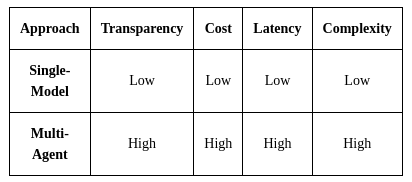
\includegraphics[width=0.5\linewidth]{images/single_vs_multi_model.png}
    \caption{Comparison of single-model and multi-agent approaches}
    \label{fig:placeholder}
\end{figure}

One of the best-known examples of this trend is HuggingGPT, introduced by Shen et al.\ \cite{shen2023hugginggpt}. In this framework, an LLM acts as a controller that delegates subtasks to external models hosted on the Hugging Face platform. The controller coordinates the results and integrates them into a final response. Liang et al.\ \cite{liang2023taskmatrix} proposed a similar system, TaskMatrix.AI, which connects LLMs with thousands of external APIs so that each subtask can be handled by the tool best suited for it. These studies show how LLMs can work as managers that coordinate specialized modules, rather than attempting to solve every step by themselves.

Other work has focused on applying multi-agent ideas directly to document and information extraction. Park et al.\ \cite{park2023generative} describe generative agents that cooperate to process documents: one agent extracts candidate entities, while another validates or reformats them according to schema constraints. This separation of roles reduces the cognitive load on any single model and makes the pipeline easier to debug, since errors can be traced back to a specific agent. Du et al.\ \cite{du2023improving} investigate multi-agent dialogue, where different agents simulate roles such as information seeker, verifier, and summarizer, in order to improve factual consistency. These ideas can be transferred to template filling, where one agent extracts fields, another checks them, and a third refines or corrects them.

Consensus-based multi-agent systems add another layer of reliability. Wu et al.\ \cite{wu2023autoagents} introduced AutoAgents, an open-source framework where multiple agents generate alternative outputs which are then compared, aggregated, or voted on. This ensemble-style approach reduces variance and improves robustness by leveraging diversity across agents. It mirrors classical redundancy methods but benefits from the contextual reasoning abilities of LLMs, making it especially useful in noisy or ambiguous input scenarios.

Despite their advantages, multi-agent systems face important challenges. They require more coordination and introduce overhead, since communication between agents can be costly and errors in one stage can still propagate. Designing reliable interfaces between agents is crucial, otherwise misalignments may cause cascading errors. In addition, evaluation of coordination quality is still underdeveloped; most benchmarks focus on the final output rather than the collaboration process itself. Finally, multi-agent pipelines often have longer latency and higher costs compared to single-model approaches.

In the context of this thesis, multi-agent systems are highly relevant because they address three requirements identified earlier: transparency, user correction, and adaptability. By splitting tasks into separate roles, they allow errors to be traced to specific stages (supporting transparency), corrections to be integrated incrementally, and domain knowledge to be embedded in specialized agents. At the same time, their higher cost and coordination complexity highlight trade-offs compared to simpler single-model systems. These trade-offs motivate the comparative evaluation carried out in this thesis, where multi-agent strategies are tested alongside monolithic and hybrid approaches.


\subsection{Evaluation of Requirements in Existing Solutions}
The reviewed approaches show steady progress in structured information extraction. Rule-based and statistical systems established transparent baselines but depended on handcrafted features and did not generalize well. Generative transformers (e.g., Du et al.\ \cite{du2021template}) enabled end-to-end template filling and improved accuracy. Speech-focused work (Sun et al.\ \cite{sun2023slot}) pushed extraction under noisy ASR inputs. Schema-centric methods and tools (Zhang et al.\ \cite{zhang2023sgptod}; Google LangExtract \cite{google2024langextract}) stabilized output formats, while constrained decoding \cite{anderson2017guided} enforced structure. Beyond extraction, Chen et al.\ \cite{le2025automated} showed schema-constrained generation for web testing. Multi-agent lines (Shen et al.\ \cite{shen2023hugginggpt}; Liang et al.\ \cite{liang2023taskmatrix}; Park et al.\ \cite{park2023generative}) introduced modularity, coordination, and validation. 

When judged against the requirements in the above Section, no single approach satisfies all of \textbf{R1--R6}. The consolidated table below summarizes what each work \emph{explicitly} supports (we mark a requirement as satisfied only if the paper/tool itself provides direct evidence; otherwise we mark ``---'' as \emph{not mentioned}).

% ===== Consolidated table (10 papers, R1--R6) =====
\begin{table*}[h!]
\centering
\renewcommand{\arraystretch}{1.25}
\setlength{\tabcolsep}{8pt}
\small
\begin{tabular}{|l|c|c|c|c|c|c|}
\hline
\textbf{Paper / Tool} & \textbf{R1} & \textbf{R2} & \textbf{R3} & \textbf{R4} & \textbf{R5} & \textbf{R6} \\
\hline
Du et al.\ 2021 \cite{du2021template} & \cmark & \cmark & \xmark & \xmark & \xmark & --- \\
Sun et al.\ 2023 \cite{sun2023slot} & \cmark & \cmark & \xmark & \xmark & \xmark & --- \\
Chen et al.\ 2025 \cite{le2025automated} & \cmark & \cmark & \xmark & \xmark & \xmark & --- \\
Google LangExtract 2024 \cite{google2024langextract} & \cmark & \cmark & \xmark & \xmark & \xmark & --- \\
Zhang et al.\ 2023 \cite{zhang2023sgptod} & \cmark & \cmark & \xmark & \xmark & \xmark & --- \\
Lin et al.\ 2021 \cite{lin2021leveraging} & \cmark & \cmark & \xmark & \xmark & \cmark & --- \\
Peng et al.\ 2023 \cite{peng2023check} & \cmark & \cmark & \xmark & \cmark & \cmark & --- \\
Shen et al.\ 2023 \cite{shen2023hugginggpt} & \cmark & \cmark & \cmark & \xmark & \cmark & --- \\
Liang et al.\ 2023 \cite{liang2023taskmatrix} & \cmark & \cmark & \xmark & \xmark & \cmark & --- \\
Park et al.\ 2023 \cite{park2023generative} & \cmark & \cmark & \cmark & \cmark & \cmark & --- \\
\hline
\end{tabular}
\caption{Consolidated evaluation of reviewed works against requirements R1--R6.}
\vspace{4pt}
\footnotesize \textit{Legend:} \cmark\,= satisfied; \xmark\,= not satisfied; ---\,= not mentioned.
\end{table*}


% ===== 2–3 lines per paper (brief evidence-based notes) =====
\paragraph{Du et al.\ 2021 \cite{du2021template}.}
End-to-end generative template filling outperforms pipelines on MUC-4 and models cross-event dependencies (R1, R2). No evidence spans, confidence scores, user correction, or adaptive learning are provided (R3--R5). Latency/usability not reported (R6).

\paragraph{Sun et al.\ 2023 \cite{sun2023slot}.}
Evaluates LLMs for slot filling from noisy ASR (SLURP), with prompt structures, LoRA, and LKI improving accuracy (R1, R2). No transparency or user-correction loop; adaptation is not defined as learning from corrections/ontologies (R3--R5). No latency reporting (R6).

\paragraph{Chen et al.\ 2025 \cite{le2025automated}.}
Combines screen transition/state graphs with LLMs to generate structured Selenium scripts (R1, R2). No interpretability, correction mechanisms, or adaptive learning (R3--R5). No runtime/latency analysis (R6).

\paragraph{Google LangExtract 2024 \cite{google2024langextract}.}
Production tool mapping text to user-defined JSON schemas with validation (R1, R2). Opaque single-model design with no interactive correction or learning from edits (R3--R5). No latency claims (R6).

\paragraph{Zhang et al.\ 2023 \cite{zhang2023sgptod}.}
Schema-guided prompting reduces invalid slot outputs in task-oriented dialogue (R1, R2). No span-level evidence, correction loop, or learning-from-corrections (R3--R5). No latency reporting (R6).

\paragraph{Lin et al.\ 2021 \cite{lin2021leveraging}.}
Slot descriptions enable zero-shot DST across unseen domains, supporting generalization (R1, R2, R5). Lacks transparency and user correction (R3, R4). No latency discussion (R6).

\paragraph{Peng et al.\ 2023 \cite{peng2023check}.}
Automated feedback improves factuality and structured outputs (R1, R2). Uses iterative prompt refinement as a correction signal and integrates external knowledge (R4, R5). No transparency or latency reporting (R3, R6).

\paragraph{Shen et al.\ 2023 \cite{shen2023hugginggpt}.}
LLM controller coordinates HF models; task planning and tool selection logs provide partial transparency (R1--R3). No explicit user-correction mechanism; adaptable via tool selection (R4, R5). No latency reporting (R6).

\paragraph{Liang et al.\ 2023 \cite{liang2023taskmatrix}.}
Connects LLMs with a large API ecosystem to perform varied tasks via structured calls (R1, R2); adaptable across domains (R5). No interpretability or correction loop (R3, R4). No latency metrics (R6).

\paragraph{Park et al.\ 2023 \cite{park2023generative}.}
Multi-agent document pipeline separates extraction and validation, improving traceability and enabling correction; modular agents support adaptation (R1--R5). No latency/usability characterization (R6).

% ===== Section wrap-up =====
\paragraph{Summary.}
Across R1--R6, current solutions contribute complementary strengths: end-to-end generative models lift accuracy; speech-focused methods add noise robustness; schema-guided designs stabilize formats; and multi-agent systems improve transparency, correction, and adaptability. Yet none meet all requirements simultaneously. This motivates the comparative experiments in later chapters, where we implement single-pass, iterative, consensus-based, and multi-agent designs and evaluate them with the same R1--R6 framework to quantify trade-offs in realistic, speech-driven scenarios.

